\documentclass{beamer}

\usepackage{polski}
\usepackage[utf8]{inputenc}
\usepackage{graphicx}
\usepackage{listings}
\usepackage{verbatim} 
\usepackage{color}
\definecolor{orange}{HTML}{FF7F00}
\lstset{
language=C,
basicstyle=\ttfamily\scriptsize,
columns=fullflexible,
keepspaces,
breaklines,
tabsize=3, 
showstringspaces=false,
extendedchars=true,
keywordstyle=\color{blue}\ttfamily,
stringstyle=\color{red}\ttfamily,
commentstyle=\color{orange}\ttfamily}

\usepackage{relsize}



%c C sharp
\def\Csharp{%
    C\kern-.1667em\raise.30ex\hbox{\smaller{\#}}%
 }

\title{Proces wytwarzania oprogramowania na platformę Windows Runtime na przykładzie aplikacji biznesowej.}   
\subtitle{Praca inżynierska}
\author{Paweł Sołtysiak} 
\institute{Promotor pracy: dr inż.  Witold Maćków\\Recenzent pracy:dr inż. Piotr Błaszyński}
\date{\today} 
\usetheme{Warsaw}

\begin{document}


\begin{frame}
\titlepage
\end{frame} 


\begin{frame}
\frametitle{Cel pracy} 
Praca dyplomowa ma na celu przedstawienie metodologii wytwarzania oprogramowania dla platformy Windows Runtime. Opisuje ona dostępne narzędzia, technologie, języki programowania oraz sposoby tworzenia interfejsu użytkownika.

Ponadto celem pracy jest stworzenie aplikacji biznesowej z wykorzystaniem zebranej wiedzy o platformie Windows Runtime.
\end{frame}


\begin{frame}
\frametitle{Zawartość pracy dyplomowej}
Praca dyplomowa została podzielona na następujące części:
\begin{itemize}[<+->]
\item Charakterystyka problemu
\item Proces wytwórczy oprogramowania
\item Wizja i projekt aplikacji Files
\item Implementacja i testy aplikacji Files
\end{itemize}
\end{frame}

\begin{frame}
\frametitle{Windows 8}
 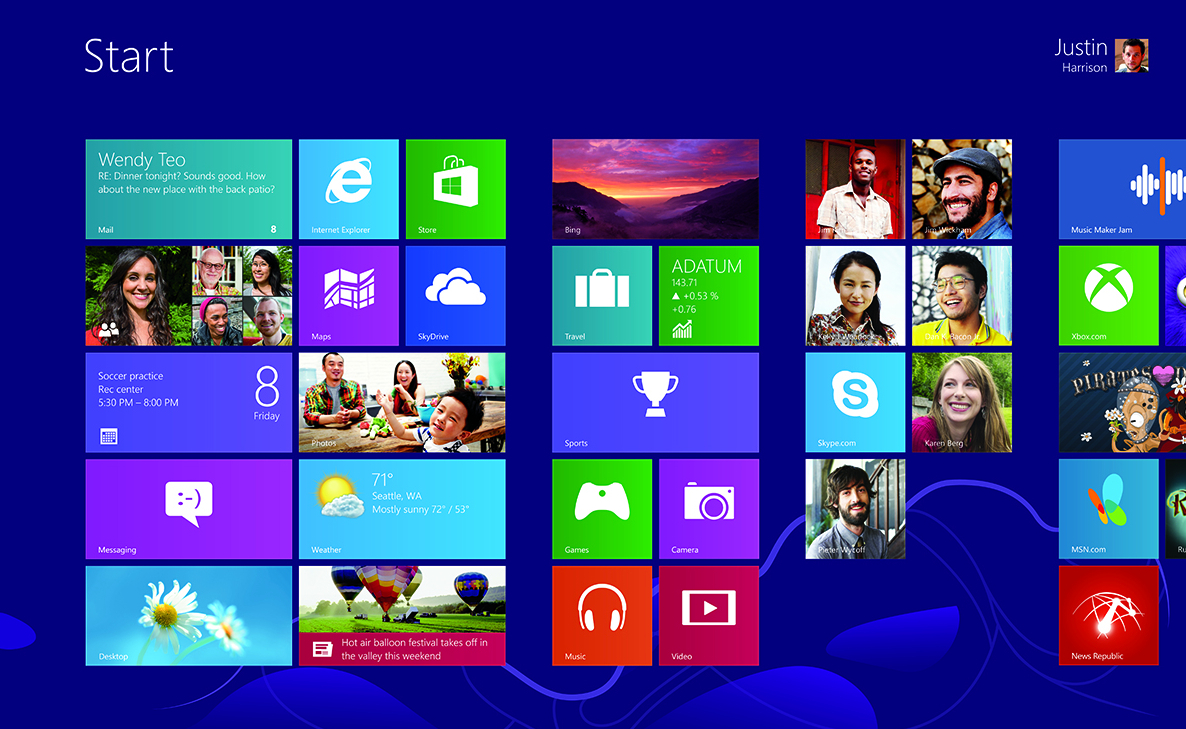
\includegraphics[width=\textwidth]{images/windows-8.jpg}
\end{frame}

\begin{frame}
\frametitle{Proces wytwórczy oprogramowania}
Proces wytwórczy oprogramowania został oparty na modelu kaskadowym (ang. Waterfall)

Etapy tworzenia oprogramowania zostały podzielone na:
\begin{itemize}[<+->]
\item Planowanie 
\item Analiza
\item Projekt
\item Implementacja 
\item Testowanie 
\item Wdrożenie
\end{itemize}
\end{frame}

\begin{frame}
\frametitle{Projekt aplikacji Files}
Podczas tworzenia projektu aplikacji zostały wykorzystane informacje przedstawione w proponowanym procesie wytwórczym oprogramowanie.

W projekcie uwzględniono
\begin{itemize}[<+->]
\item Wymagania funkcjonalne i niefunkcjonalne
\item Schematy pokazujące funkcjonowanie aplikacji
\item Model danych aplikacji
\item Analizę wykorzystanych narzędzi
\item Opisano strukturę logiczną aplikacji
\end{itemize}
\end{frame}

\begin{frame}
\frametitle{Implementacja aplikacji Files}
Podczas tworzenia implementacji aplikacji zachowano wszystkie założenia przedstawione wcześniej w pracy.

\end{frame}

\begin{frame}
\maketitle
\end{frame}

\end{document}
